\documentclass[11pt]{amsart}

\usepackage[utf8]{inputenc}
\usepackage[spanish]{babel}
\usepackage{enumerate}
\usepackage{graphicx}
\usepackage{hyperref}
\usepackage[vmargin=2cm,hmargin=2cm]{geometry}

%en corchetes ponemos nombres más cortos, para mejor visualización de las cabeceras del documento
\title[Taller de \LaTeX]{Taller de \LaTeX\ en el Instituto de Biomedicina del Campus de la Salud}
\author[Los presentes]{Los asistentes a dicho curso}
\thanks{Agradecemos a la oficina de software libre que organice estos eventos}

\address{Instituto de Biomedicina}
\email{alguno@ugr.es}
\date{\today}
\keywords{\LaTeX, taller software libre}

\begin{document}

%para mostrar los acentos hemos puesto \usepackage[utf8]{inputenc} en la cabecera
%para que aparezca "Resumen" en vez de "Abstract" usamos \usepackage[spanish]{babel}, esto afecta a muchas otras variables, que ahora aparecerán en español
\begin{abstract}
Esto es una prueba de cómo hacer algunas cosas en \LaTeX. 
\end{abstract}

%con este comando le indicamos a LaTeX que produzca el título con los autores y resumen. En algunos estilos, la dirección aparece también en la primera página.
\maketitle

%esta orden genera un índice
\tableofcontents


%los comandos con asterisco evitan la numeración
\section*{Introducción}

Este taller está pensado como pequeña introducción al \LaTeX. Intentaremos dar algunas pequeñas pinceladas sobe su uso. Para m\'as detalles véase \cite{lshort}.
%con \cite hacemos una referencia, que tendrá que estar definida en la sección de la bibliografía (véase el final del fichero)

\section{Listas}

Hay varios tipos de listas.
%gracias al paquete 'enumerate' podemos especificar cómo son los índices usados para enumerar
\begin{enumerate}[1)]
\item Aquellas que van enumeradas.
	\begin{enumerate}
	\item \ldots que además se pueden anidar.
	\end{enumerate}

\item Aquellas sin enumerar:
\begin{itemize}
\item[$\diamond$] damos varios apartados, %entre corchetes puedo indicar el símbolo que inicia la frase
\begin{itemize}
\item y podemos también anidar.
\end{itemize}
\end{itemize}
\end{enumerate}


\section{Tablas} 

Un ejemplo simple de tabla.

%lcr significa que hay tres columnas, la primera justificada a la izquierda (l), la segunda al centro y la última a la derecha
\begin{tabular}{lcr}
1 & 2 & 3 \\
Pepe & Juan & Manuel
\end{tabular}

Y otra un poco más elaborada.

%las separaciones verticales se hacen con | en la especificación del número y justificación de columnas
%las líneas verticales se consiguen con \hline
\begin{tabular}{l||c|c|c|} \hline
Posición & 1 & 2 & 3 \\ \hline \hline
Nombre & Pepe & Juan & Manuel\\ \hline
\end{tabular}


\section{Algunos tipos de letra, que no tipografías}

Podemos escribir en  \textbf{negrita}, en \textit{itálica}, en \textsl{helvética}, en \texttt{courier}, en \textsc{pequeñas MayúsculaS} ... o bien podemos \emph{enfatizar} una \textit{parte del texto \emph{dentro} de otro}.

Podemos decir las cosas en {\large alto}, o más {\Large alto}, o incluso {\huge más} fuerte {\Huge aún}.


\section{Fórmulas}

Básicamente hay dos tipos de fórmulas.
\begin{itemize}
\item Aquellas que van insertadas en el texto, como por ejemplo $2^{x+y}\int_a^b e^{\frac{x^2}{2}}\lim_{x\to 1}x^{x-1}$.
\item Otras que se ponen en modo pantalla (\emph{display}): \[\max\{2^{x+y}\int_a^b e^{\frac{x^2}{2}}\lim_{x\to 1}x^{x-1},1\}.\]
Compárese esta última con 
\[\max\left\{2^{x+y}\int_a^b e^{\frac{x^2}{2}}\lim_{x\to 1}x^{x-1},1\right\}.\]
\end{itemize}

También podemos poner fórmulas con etiquetas,
\begin{equation}\label{formula} %acabamos de ponerle una etiqueta a la fórmula 
\sum_{i=1}^n i=\frac{n(n+1)}2,
\end{equation}
para poder referirnos a ellas más tarde (por ejemplo: la fórmula \ref{formula} se verifica para todo $n$ entero positivo). %con ref hacemos referencia a una etiqueta definida en otro sitio del texto

\section{Algunos entornos}

%el primer argumento es el nombre del entorno, el segundo el número de parámetros que le pasamos, el tercero indica cómo empieza el entorno, y el último cómo termina (en este caso terminamos con un cuadrado hueco)
\newenvironment{ejercicio}[1]{\textbf{Ejercicio número #1}}{\qed}

Veamos cómo escribir un ejercicio.

\begin{ejercicio}{1}
Escribe esto con otras palabras.
\end{ejercicio}

Otra forma con contadores.
%definimos un contador, así no tenemos que poner manualmente número a los ejercicios
\newcounter{ejer_num}
%ponemos el contador a 1
\setcounter{ejer_num}{1}
%definimos ahora un nuevo entorno, sin parámetros; el contador se incrementa con \stepcounter{}
\newenvironment{ejer}{\textbf{Ejercicio \arabic{ejer_num}: \stepcounter{ejer_num}}\begin{itshape}}{\end{itshape}}

\begin{ejer}
Una de melón.
\end{ejer}

\begin{ejer}
Otra de sandía.
\end{ejer}

\subsection{Otros entornos}

%el entorno teorema irá numerado usando las secciones con el formato (nºsección).(nºteorema en la sección)
\newtheorem{teorema}{Teorema}[section]
%con esta forma de definir nota, hacemos que tenga el mismo tipo de contador que el entorno teorema anteriormente definido
\newtheorem{nota}[teorema]{Aclaración}

\begin{teorema}\label{tonto}
Las ranas son verdes.
\end{teorema}
%el entorno proof está predefinido en amsart, al usar el paquete babel con la opción spanish, imprimirá "Demostración:" en vez de "Proof:".
\begin{proof}
Así lo decía Aristóteles, y nosotros no vamos a llevarle la contraria.
\end{proof}

\begin{nota}
Alguien probó que el Teorema \ref{tonto} es falso, pues encontró una rana marrón.
\end{nota}


\section{Imágenes}

%las figuras son entornos flotantes, se colocarán donde mejor encajen en el documento final
\begin{figure}
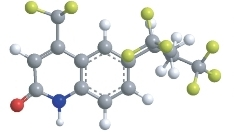
\includegraphics[width=3cm]{imagen.jpg}  %esta orden indica que ponemos aquí la imagen del fichero "imagen.jpg" con una anchura de 3cm; otros parámetros son scale, height...
\caption{Algo que encontré por %con esta orden determinamos el texto que acompaña a la figura
\href{http://www3.interscience.wiley.com/journal/13087/home/ForAuthors.html}{ahí.}%gracias al paquete hyperref, podemos poner enlaces a páginas en internet
}
\label{uno} 
\end{figure}

%las minipáginas son útiles para definir páginas más pequeñas dentro de otras; aquí aparecen dos una detrás de la otra, y la segunda empujada hacia la derecha por un \hfill
\begin{minipage}{8cm}
En la Figura \ref{uno} se puede ver una imagen. O bien podemos ponerla aquí a la derecha. 
\end{minipage} 
\hfill \begin{minipage}{3cm}
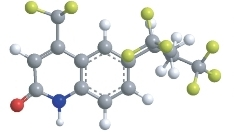
\includegraphics[width=2.5cm]{imagen.jpg}
\end{minipage}



\section{Definiciones}

\newcommand{\Z}{{\mathbb Z}}
\newcommand{\f}[2]{{\int_0^\infty #1 d #2}}

Si se usa mucho un objeto, se puede definir un comando que imprima ese objeto. Por ejemplo ``$\Z$ denota el conjunto de los enteros, y tomemos un elemento $x\in \Z$''. O bien si vamos a calcular muchas integrales de un mismo tipo: $\f{x^2}{x}$, $\f{e^{xy^2}}{y}$, \ldots



\section{Moviendo texto}

\begin{center}
Con esto termina el curso, si queréis más, sólo tenéis que pedirlo.

Gracias por vuestra atención.
\end{center}

\hfill Hasta pronto.


%el número 10 no es significativo, realmente dice que el número de citas es un número de a lo sumo dos dígitos
\begin{thebibliography}{10}
\bibitem{lshort} Tobias Oetiker, Hubert Partl, Irene Hyna and Elisabeth Schlegl, The not so short introduction to \LaTeX2e, \href{http://www.ctan.org/tex-archive/info/lshort/english/lshort.pdf}{ctan.org}.
\end{thebibliography}

\end{document}